% CREATED BY MAGNUS GUSTAVER, 2020
\chapter{Testing protocol} \label{testingProtocol}

The following appendix documents tests that have been performed during the project. They are documented in such a way that they can be repeated to validate the functionality of the balancing algorithm on either this or another version of the Autobike in the future.

\section{Angular velocity of the Forward Motor Follows the Setpoint Value}

To test that the Angular velocity of the forward motor follows the setpoint value, the \textit{Auto Tuning} feature in ESCON Studio was used. The results presented in the image below are that the actual speed (red line) follows the setpoint speed (blue line), with the exception of the initial acceleration and deceleration. 

\begin{figure}[h]
    \centering
    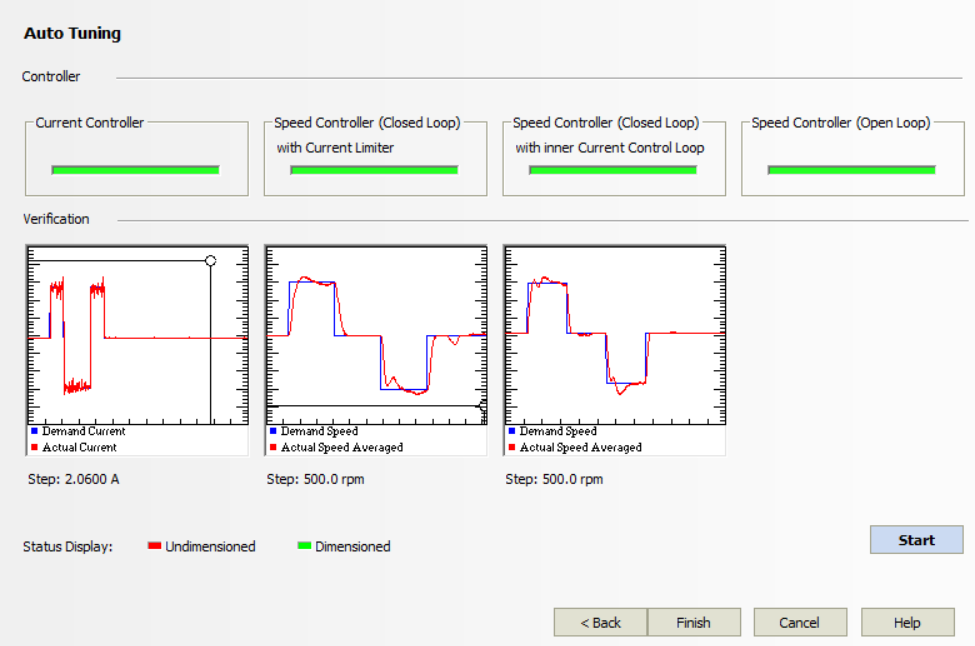
\includegraphics[width=\textwidth-2cm]{figure/esconAutoTuning.png}
    \caption{The results page after running the Auto Tuning in ESCON Studio.}
\end{figure}

\section{Duty Cycle Compared With the Angular Velocity of the Front Wheel}

In this test, the bike was lifted into the air and the balancing algorithm was bypassed so that the duty cycle sent to the steering motor could be controlled directly. The angle limit was also bypassed, so that the motor could spin freely several revolutions. The duty cycle was then set to 0.4, and the velocity of the steering motor was recorded. This velocity is also the speed that the bikes handlebar turns with, since the gear ratio between the handlebar and the motor is 1:1. The test was then repeated, but with the duty cycle set to 0.3, 0.2, and 0.1.

The initial result from this test was that the motor took 8 seconds to accelerate from stationary to the maximum velocity as seen in image \ref{fig:pwmVelocityTest}. This was later fixed by uploading the ESCON configuration from the black bike as described in \ref{methods:configESCON}. The fixed result is plotted in \ref{fig:pwmVelocityTestFixed}.

\begin{figure}[H]
    \begin{subfigure}{.5\textwidth}
        \centering
        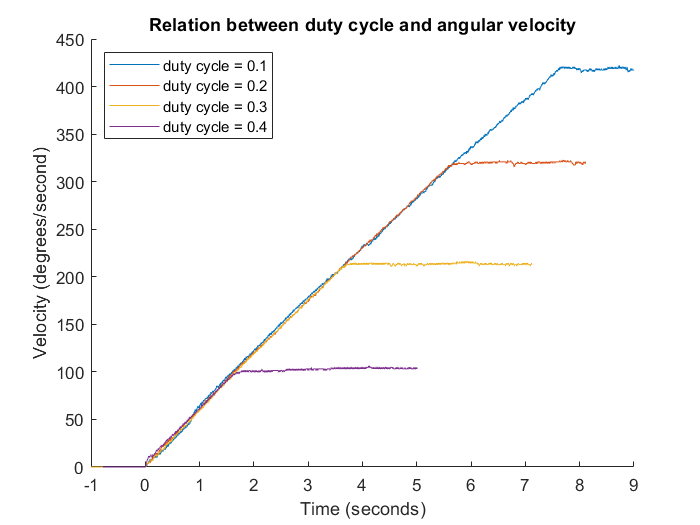
\includegraphics[width=\textwidth]{figure/pwmVsVelocity.png}
        \caption{Duty cycle vs velocity with the wrong motor configuration.}
        \label{fig:pwmVelocityTest}
    \end{subfigure}
    \begin{subfigure}{.5\textwidth}
        \centering
        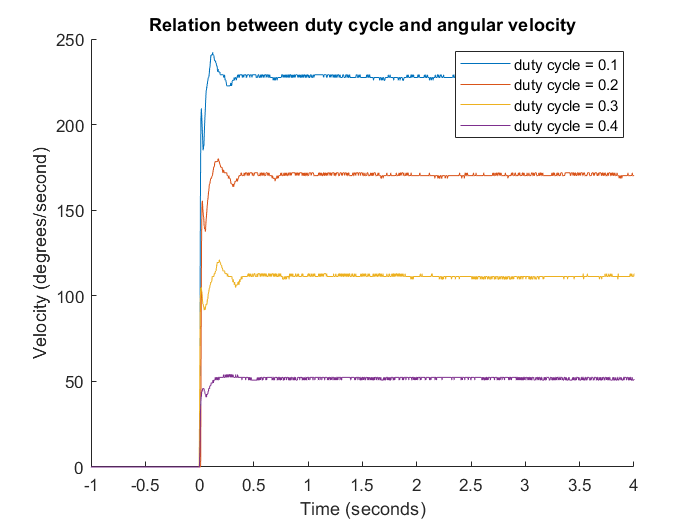
\includegraphics[width=\textwidth]{figure/pwmVsVelocityFixed.png}
        \caption{The position and velocity of steering motor.}
        \label{fig:pwmVelocityTestFixed}
    \end{subfigure}
\caption{Test results of varying duty cycles compared with the angular velocity of the steering motor.}
\end{figure}

\newpage

\section{Gyroscope Measurements When Tilting the Bike}

This test was performed by tilting the bike back and forth. While logging the data from the gyroscope for each axis. Before performing these tests, the mount for IMU had been fixed so that the IMU was no longer placed at an angle. The data from the test is illustrated in the figure below. 

What can be seen is that the Z-axis is the axis which is affected the most. This is also the axis which should be affected by tilting the bike side to side. It can also be seen that the Y-axis has some very minor movements, which is because the current mount is not very exact, and it is difficult to precisely adjust the placement angle.

\begin{figure}[h]
    \centering
    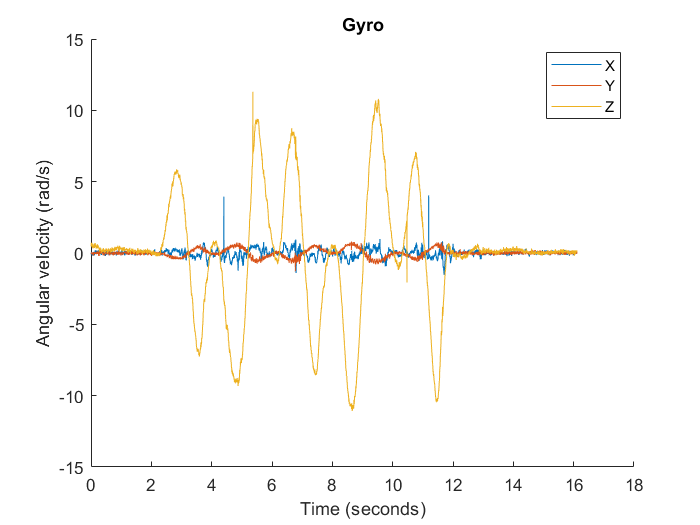
\includegraphics[width=\textwidth]{figure/gyroAlignmentTest.png}
\end{figure}

\newpage

\section{Gyroscope and Position}

This test was performed by leaning the bike towards a wall and measuring the angle the electronics box has when it touches the wall; in this case the angle was 20\degree. The bike was then leaned from an upright position until it hit the wall, whilst the data from the gyroscope for each axis was logged. The data from this test is illustrated in the figure below, together with the integral of the gyroscope's data for the Z-axis, which corresponds with how much the bike has been tilted.

The maximum angle of the bike is recorded as -11 radians, when it should have been $20 * \frac{\pi}{180} \approx 0.35$ radians. The conclusion which can be made from this is that the gyro recordings are wrong with a factor of $\frac{11}{0.35} = 31.4$. The reason for this could not be found, so to compensate for the error, all readings were divided by 31.4 inside of the LabVIEW program before being used in any calculations.

\begin{figure}[h]
    \centering
    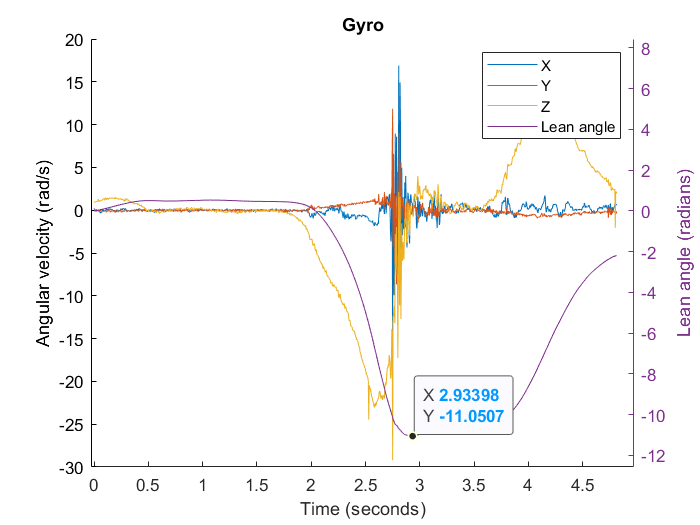
\includegraphics[width=\textwidth]{figure/gyroAngleTestWrong.png}
\end{figure}

\newpage

\subsection{After Multiplying With the Calculated Factor}

The next test was performed after the factor which compensates for the error was added. The test was otherwise performed exactly as the previous test, the only difference being the measured angle was 16\degree. The data from the test is shown in the figure below.

This graph shows that the maximum angle is -0.288 radians, or 16.5\degree. The values of the angular velocities is also more reasonable. All future tests presented below have also been performed with the the correcting factor of 31.4.

\begin{figure}[h]
    \centering
    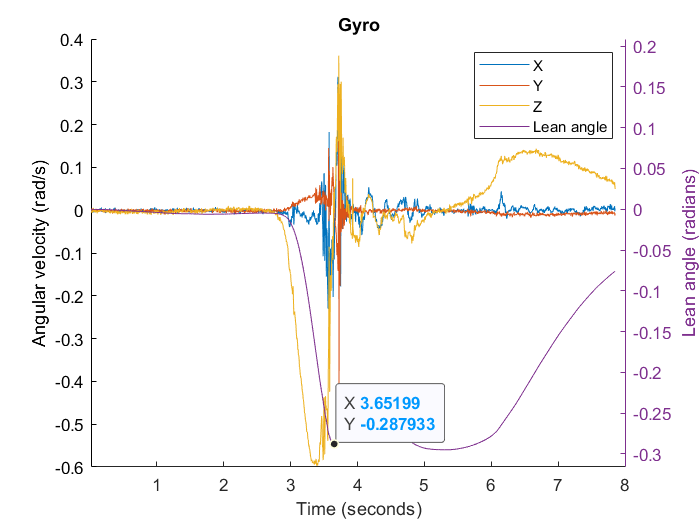
\includegraphics[width=\textwidth]{figure/gyroAngleTestCorrected.png}
\end{figure}

\newpage

\section{Duty Cycle Compared With the Gyroscope's Measurements}

This test was performed by allowing the bike to naturally fall a few centimeters, before catching it. The roll rate (data from the Z-axis of the gyroscope), together with the duty cycle given by the balancing algorithm is displayed in the figure below. During this test, the P gain of the balancing controller was set to 1.

The result from this test is that the duty cycle follows the roll rate almost perfectly. It also never reaches the upper and lower limits of 0.9 and 0.1 respectively.

\begin{figure}[h]
    \centering
    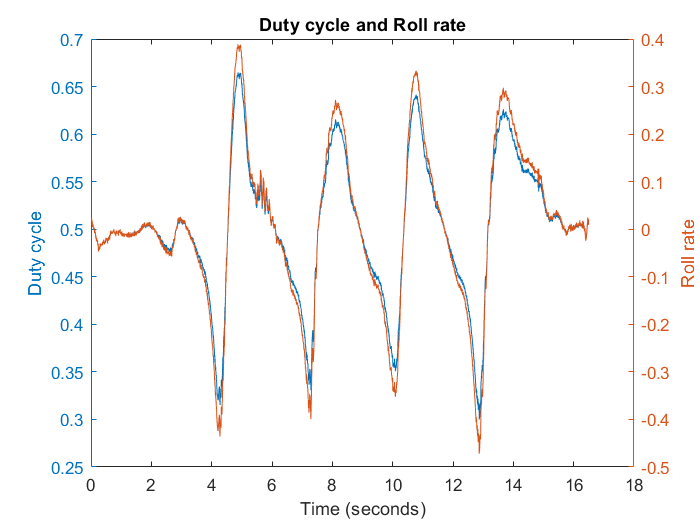
\includegraphics[width=\textwidth]{figure/pwmVsRollRate.png}
\end{figure}

\newpage

\subsection{After Adjusting the Balancing Algorithm}

This test was performed exactly as the previous one. The difference being the balancing algorithm had been changed so that the maximum duty cycle of 0.9 is only reached when the roll rate multiplied with the P gain is the same as the steering motor's maximum angular velocity, which is set to 4000 RPM in ESCON Studio. This is how the algorithm is indented to work. The upcoming figure illustrates the data from the test.

In the data below, it can be seen that the duty cycle is much lower for the same roll rates. This can be affected by increasing the P gain of the balancing controller.

\begin{figure}[h]
    \centering
    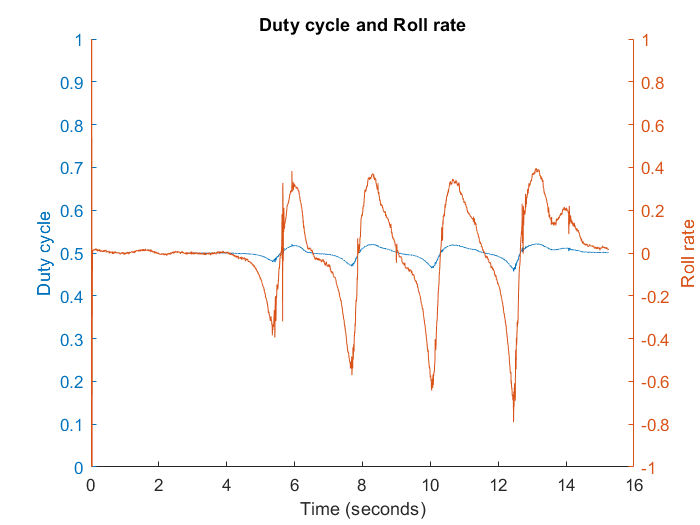
\includegraphics[width=\textwidth]{figure/pwmVsRollRateCorrected.png}
\end{figure}

\newpage

\section{Unaided Outdoor Test}

When performing the final tests outdoors in an open area, the motor controller for the forward motor (the VESC) was broken (this is further discussed in section \ref{results:discussion}), so the bike had to be pushed by hand. The test was started by enabling the steering motor, pushing the bike up to speed and then letting it go. The P gain of the balancing algorithm was initially set to 1. This resulted in the bike having close to no control response, which lead to it falling over and having to be caught within a second after letting go.

The P gain was then increased to 5, and the test was repeated. The results of this can be seen in figure \ref{fig:outdoorTest}. Here it is shown that the roll rate as well as the duty cycle is close to their center throughout the test, except for around the 25:th second when the bike drove over a bump. It can also be seen that the duty cycle reacts to the roll rate and that the steering motor follows the duty cycle.

\begin{figure}[H]
    \begin{subfigure}{.5\textwidth}
        \centering
        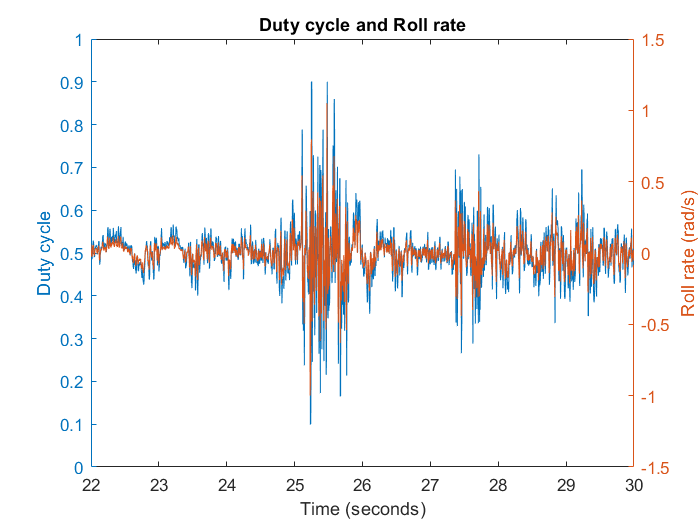
\includegraphics[width=\textwidth]{figure/dutyAndRoll.png}
        \caption{Duty cycle and the roll rate of the bike.}
    \end{subfigure}
    \begin{subfigure}{.5\textwidth}
        \centering
        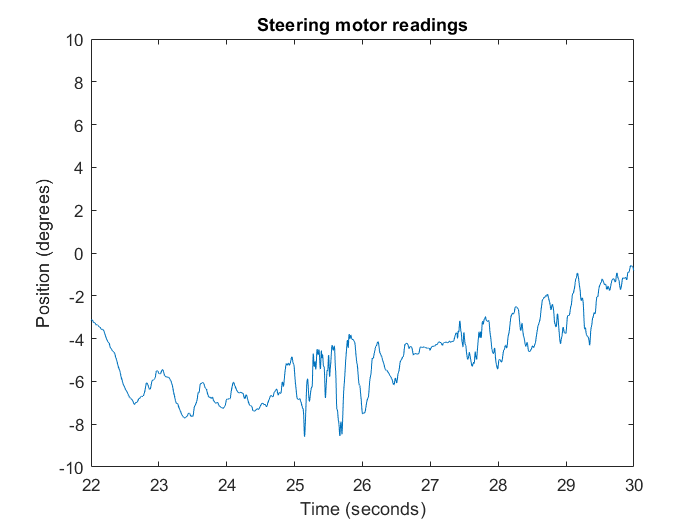
\includegraphics[width=\textwidth]{figure/motorPosition.png}
        \caption{The position of the forward motor.}
    \end{subfigure}
\caption{The final test results of running the bike outside on an open area.}
\label{fig:outdoorTest}
\end{figure}